\documentclass{beamer}
\usepackage[utf8]{inputenc}

\usetheme{Madrid}
\usecolortheme{default}
\usepackage{amsmath,amssymb,amsfonts,amsthm}
\usepackage{txfonts}
\usepackage{tkz-euclide}
\usepackage{listings}
\usepackage{adjustbox}
\usepackage{array}
\usepackage{tabularx}
\usepackage{gvv}
\usepackage{lmodern}
\usepackage{circuitikz}
\usepackage{tikz}
\usepackage{graphicx}
\setbeamertemplate{page number in head/foot}[totalframenumber]
\usepackage[T1]{fontenc}
\usepackage{tcolorbox}
\tcbuselibrary{minted,breakable,xparse,skins}

\definecolor{bg}{gray}{0.95}
\DeclareTCBListing{mintedbox}{O{}m!O{}}{%
  breakable=true,
  listing engine=minted,
  listing only,
  minted language=#2,
  minted style=default,
  minted options={%
    linenos,
    gobble=0,
    breaklines=true,
    breakafter=,,
    fontsize=\small,
    numbersep=8pt,
    #1},
  boxsep=0pt,
  left skip=0pt,
  right skip=0pt,
  left=25pt,
  right=0pt,
  top=3pt,
  bottom=3pt,
  arc=5pt,
  leftrule=0pt,
  rightrule=0pt,
  bottomrule=2pt,
  toprule=2pt,
  colback=bg,
  colframe=orange!70,
  enhanced,
  overlay={%
    \begin{tcbclipinterior}
    \fill[orange!20!white] (frame.south west) rectangle ([xshift=20pt]frame.north west);
    \end{tcbclipinterior}},
  #3,
}

% Code style
\lstset{
    language=C,
    basicstyle=\ttfamily\small,
    keywordstyle=\color{blue},
    stringstyle=\color{orange},
    commentstyle=\color{green!60!black},
    numbers=left,
    numberstyle=\tiny\color{gray},
    breaklines=true,
    showstringspaces=false,
}

% Title info
\title %optional
{4.2.16}
\date{October 3, 2025}
\author % (optional)
{EE25BTECH11018 - Darisy Sreetej}

\begin{document}

\frame{\titlepage}

\begin{frame}{Question}
Let $a, b, c ,d$ be non-zero numbers. If the point of intersection of the lines $4a\vec{x} +2a\vec{y} + c = 0$ and $5b\vec{x} + 2b\vec{y} + d = 0$ lies in the fourth quadrant and is equidistant from the two axes then
\begin{enumerate}
    \item $3bc-2ad=0$
    \item $2bc-3ad=0$
    \item $3bc+2ad=0$
    \item $2bc+3ad=0$
\end{enumerate}
\end{frame}
\begin{frame}{Solution}
The two lines are
\begin{align}
4a\vec{x} +2a\vec{y} + c = 0  , \\
5b\vec{x} + 2b\vec{y} + d = 0 
\end{align}
According to the condition,the intersection point is equidistant from the axes and lies in the fourth quadrant, so its coordinates satisfy $y=-x$ \\
\begin{align}
\vec{x}+\vec{y}=0
\end{align}
This equation can be expressed in terms of matrices
\begin{align}
\myvec{4a\\2a}^\top\myvec{\vec{x}\\\vec{y}}=-c\\
\myvec{5b\\2b}^\top\myvec{\vec{x}\\\vec{y}}=-d
\end{align}
\end{frame}
\begin{frame}{Solution}
\begin{align}
    \myvec{1\\1}^\top\myvec{\vec{x}\\\vec{y}}=0
\end{align}
They can be represented as,
\begin{align}
    \myvec{4a&5b\\2a&2b\\1&1}^\top\myvec{\vec{x}\\\vec{y}}=\myvec{-c\\-d\\0}
\end{align}
Using augmented matrix,
\begin{align}
\augvec{2}{1}{4a&2a&-c\\5b&2b&-d\\1&1&0}
\end{align}
$R_3=R_3-4aR_1$\\
$R_2=R_2-5bR_1$
\end{frame}
\begin{frame}{Solution}
\begin{align}
\augvec{2}{1}{1&1&0\\0&-3b&-d\\0&-2a&-c}
\end{align}
$R_3=R_3-\frac{2a}{3b}R_2$
\begin{align}
\augvec{2}{1}{1&1&0\\0&-3b&-d\\0&0&-c+\frac{2ad}{3b}}
\end{align}
\begin{align}
\augvec{2}{1}{1&1&0\\0&-3b&-d\\0&0&\frac{2ad-3bc}{3b}}
\end{align}
The last row of the matrix represents the equation
\begin{align}
\vec{y}0+\vec{x}0=\frac{2ad-3bc}{3b}
\end{align}
\end{frame}
\begin{frame}{Solution}
For the system to be consistent(i.e., to have a solution),the right-hand side must be zero.
\begin{align}
\frac{2ad-3bc}{3b}=0
\end{align}
\begin{align}
2ad-3bc=0
\end{align}
Therefore,
\begin{align}
3bc=2ad
\end{align}
Therefore, option(a) is correct\\
For the point of intersection , solve the equations from (11),\\
The point of intersection is 
\begin{align}
    \myvec{\vec{x}\\\vec{y}}=\myvec{\frac{-d}{3b}\\\frac{d}{3b}}
\end{align}
\end{frame}
\begin{frame}{Solution}
   Also ,
\begin{align}
 \myvec{\vec{x}\\\vec{y}}=\myvec{\frac{-c}{2a}\\\frac{c}{2a}}  \quad (from (15))
\end{align}
It can be clearly verified by the plot
\end{frame}
\begin{frame}{Plot}
    \centering
    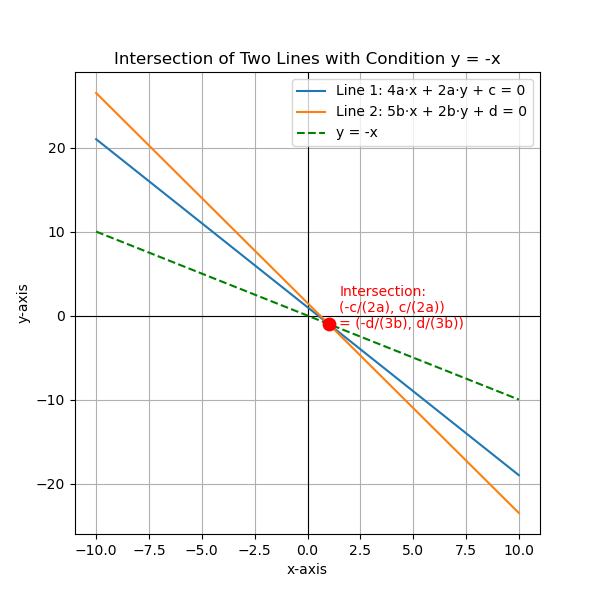
\includegraphics[width=3\columnwidth, height=0.8\textheight, keepaspectratio]{figs/fig.png}     
\end{frame}

\begin{frame}[fragile]
\frametitle{C code}
    \begin{lstlisting}[language=C]
#include <stdio.h>

// Function to compute x from first line
double computeX1(double a, double c) {
    return -c / (2.0 * a);
}

// Function to compute x from second line
double computeX2(double b, double d) {
    return -d / (3.0 * b);
}
\end{lstlisting}
\end{frame}
\begin{frame}[fragile]
    \frametitle{C Code }
    \begin{lstlisting}[language=C]
// Function to compute y (since y = -x for equidistant from axes in 4th quadrant)
double computeY(double x) {
    return -x;
}

// Function to check relation 3bc - 2ad = 0
int checkRelation(double a, double b, double c, double d) {
    double relation = 3*b*c - 2*a*d;
    return (relation == 0) ? 1 : 0;
}


     \end{lstlisting}
\end{frame}
\begin{frame}[fragile]
    \frametitle{Python + C Code }
    \begin{lstlisting}[language=Python]
import ctypes
import matplotlib.pyplot as plt
import numpy as np

# Load the compiled C shared library
lib = ctypes.CDLL("./point.so")

# Set argument and return types
lib.computeX1.argtypes = [ctypes.c_double, ctypes.c_double]
lib.computeX1.restype = ctypes.c_double

lib.computeX2.argtypes = [ctypes.c_double, ctypes.c_double]
lib.computeX2.restype = ctypes.c_double

lib.computeY.argtypes = [ctypes.c_double]
lib.computeY.restype = ctypes.c_double

lib.checkRelation.argtypes = [ctypes.c_double, ctypes.c_double, ctypes.c_double, ctypes.c_double]

    \end{lstlisting}
\end{frame}

\begin{frame}[fragile]
    \frametitle{Python + C code}

    \begin{lstlisting}[language=Python]
lib.checkRelation.restype = ctypes.c_int

# Example values (you can change these)
a, b, c, d = 1.0, 1.0, -2.0, -3.0

# Call C functions
x1 = lib.computeX1(a, c)
x2 = lib.computeX2(b, d)

if abs(x1 - x2) > 1e-6:
    print("Inconsistent intersection: x1 != x2")
    exit()

x = x1
y = lib.computeY(x)

print(f"Intersection Point: ({x:.3f}, {y:.3f})")

    \end{lstlisting}
\end{frame}

\begin{frame}[fragile]
    \frametitle{Python + C code}

    \begin{lstlisting}[language=Python]
# Check relation
if lib.checkRelation(a, b, c, d):
    print("Relation satisfied: 3bc - 2ad = 0 ")
    else:
    print("Relation NOT satisfied ")

# ---------- Plotting ----------
X = np.linspace(-10, 10, 400)

# Line1: 4ax + 2ay + c = 0 -> y = -(4aX + c)/(2a)
Y1 = -(4*a*X + c) / (2*a)

# Line2: 5bx + 2by + d = 0 -> y = -(5*bX + d)/(2*b)
Y2 = -(5*b*X + d) / (2*b)

plt.figure(figsize=(6,6))
plt.axhline(0, color="black", linewidth=0.8)
plt.axvline(0, color="black", linewidth=0.8)
\end{lstlisting}
\end{frame}
\begin{frame}[fragile]
    \frametitle{Python + C code}
    \begin{lstlisting}[language=Python]
plt.plot(X, Y1, label="Line 1")
plt.plot(X, Y2, label="Line 2")
plt.scatter([x], [y], color="red", s=80, label="Intersection Point")

plt.title("Intersection of Two Lines")
plt.xlabel("x-axis")
plt.ylabel("y-axis")
plt.legend()
plt.grid(True)
plt.show()
      \end{lstlisting}
\end{frame}
\begin{frame}[fragile]
    \frametitle{Python code}
    \begin{lstlisting}[language=Python]

import matplotlib.pyplot as plt
import numpy as np

# Example coefficients (you can change these)
a, b, c, d = 1.0, 1.0, -2.0, -3.0

# Intersection point (from condition y = -x)
x = -c / (2 * a)
y = -x

# Create range of x values for plotting
X = np.linspace(-10, 10, 400)

# Line1: 4ax + 2ay + c = 0 -> y = -(4aX + c)/(2a)
Y1 = -(4 * a * X + c) / (2 * a)

# Line2: 5bx + 2by + d = 0 -> y = -(5 * b * X + d) / (2 * b)
Y2 = -(5 * b * X + d) / (2 * b)
    \end{lstlisting}
\end{frame}
\begin{frame}[fragile]
    \frametitle{Python code}

    \begin{lstlisting}[language=Python]
# y = -x line
Y_diag = -X

# ---------- Plot ----------
plt.figure(figsize=(6, 6))
plt.axhline(0, color="black", linewidth=0.8)  # x-axis
plt.axvline(0, color="black", linewidth=0.8)  # y-axis

plt.plot(X, Y1, label="Line 1: 4a·x + 2a·y + c = 0")
plt.plot(X, Y2, label="Line 2: 5b·x + 2b·y + d = 0")
plt.plot(X, Y_diag, "g--", label="y = -x")

# Mark intersection point with symbolic label
plt.scatter([x], [y], color="red", s=80, zorder=5)
plt.text(x + 0.5, y - 0.5,
         "Intersection:\n(-c/(2a), c/(2a))\n= (-d/(3b), d/(3b))",
         fontsize=10, color="red")
           \end{lstlisting}
\end{frame}
\begin{frame}[fragile]
    \frametitle{Python code}

    \begin{lstlisting}[language=Python]
plt.title("Intersection of Two Lines with Condition y = -x")
plt.xlabel("x-axis")
plt.ylabel("y-axis")
plt.legend(loc="best")
plt.grid(True)
plt.show()
    \end{lstlisting}
\end{frame}
\end{document}
